\subsection{Neural Network Structure}
Neural networks generally have the same constitutive elements, mixed and matched based on the desired performance and complexity of the model that you are trying to build.

\subsubsection{Neural Network Building Blocks}
Generally, neural networks are formed by collections of foundational units, which can generate increasingly complex architectures and yield incredible performance. However, it is always important to start with the fundamental ``atoms'' of the neural network.

The most basic unit of a neural network is the perceptron (or neuron), which is composed of a summation of inputs multiplied by weights, a bias term, and a (typically non-linear) activation function (\cref{fig:neuron}, \cref{eq:neuron}).
\begin{figure}[h!]
    \begin{center}
        {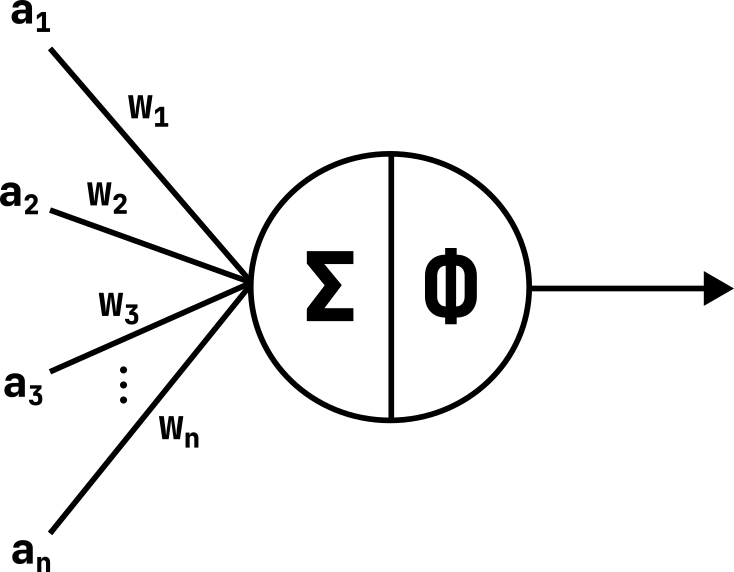
\includegraphics[width=0.55\linewidth]{figs/background/png/neuron.png}}
    \end{center}
    \caption{A schematic representing a single neuron that receives $n$ inputs and applies $\phi$ as an activation function.}
    \label{fig:neuron}
\end{figure}

\begin{equation}
    y = \phi(\sum_{i=1}^{n}a_i w_i + b)
    \label{eq:neuron}
\end{equation}

Activation functions are a crucial component in neural networks as they allow for the introduction of non-linearity, which is essential for the network's ability to learn complex representations of the input data.
Without activation functions, a neural network would only be able to learn linear relationships between the input and output.
However, many real-world problems involve non-linear relationships that cannot be captured by a linear model alone.
Activation functions provide a way to move beyond a linear relationship, allowing the neural network to learn more nuanced mappings between the input and output.
The choice of activation function depends on the specific problem you are trying to solve and the architecture of your network.
Some activation functions introduce more non-linearity than others and some trade-off between non-linearity and computational efficiency.
Experimenting with different activation functions and observing the impact on the network's performance can be a useful technique for optimizing the performance of a neural network.
A list of common activation functions and their equations is shown in Table \ref{tab:activation-functions}.

\begin{table}[H]
    \caption{A list of activation functions and their corresponding mathematical formula} \label{tab:activation-functions}
    \begin{tabularx}{\columnwidth}{|X|X|X|}
        \hline
        {\bf Activation Function} & {\bf Equation} \\ \hline 
        Linear & $\phi(x) = x$ \\\hline
        Sigmoid & $\phi(x) = \frac{e^{x}}{1 + e^{x}}$\\ \hline 
        Hyperbolic Tangent & $\phi(x) = \frac{e^x - e^{-x}}{e^{x} + e^{-x}}$\\ \hline 
        Rectified Linear Unit (ReLU) & $\phi(x) = \text{max}(0,x)$\\ \hline 
        Leaky ReLU & $\phi(x) = \text{max}(0.1x,x)$ \\ \hline 
    \end{tabularx}
\end{table}

\subsubsection{Fully Connected Network}
The fully connected network, also known as the multi-layer perceptron, is a basic type of neural network that utilizes the neurons previously discussed as building blocks.
Its schematic representation is a familiar image to many when considering neural networks.
By stacking the summations and multiplications of each neuron, we can derive the equation for a single layer of a fully connected network, which is simply a matrix multiplication (\cref{eq:fcn}).
In this equation, $W$ represents the collection of weights for each neuron, $a$ represents the input, $b$ represents the bias, and $\phi$ represents the activation function.

One of the key strengths of this type of network is the utilization of non-linear activation functions. A well-chosen activation function can greatly impact the network's performance and ability to achieve specific tasks. For example, in a binary classification task, the sigmoid activation function can be used at the output layer, constraining the output between $0$ (false) and $1$ (true). The output can then represent the probability of the given input being classified as 'true'. The ReLU activation function is another popular choice because it is computationally efficient and often used in hidden layers of deep networks. Additionally, the hyperbolic tangent (tanh) activation function is used in the context of a model where data follows a Gaussian distribution.

\begin{figure}[h!]
    \centering
    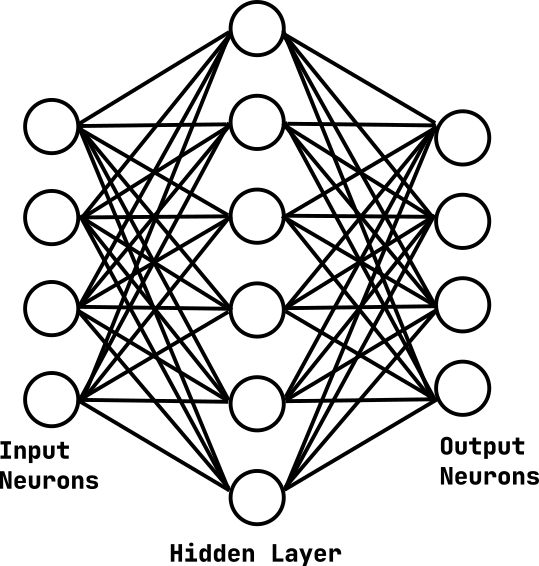
\includegraphics[width=0.7\linewidth]{figs/background/png/fcn.png}
    \caption{A basic fully connected network with a single hidden layer. Each of the neurons are exactly the same as the neurons shown in figure \ref{fig:neuron}}
    \label{fig:fcn}
\end{figure}

\begin{equation}
    y = \phi(W^{T}a + b)
    \label{eq:fcn}
\end{equation}

Additional layers can be added by taking the output of one layer and sending that into the input of the next. Increasingly complex mappings can be generated by increasing either the size or the number of hidden layers in a network.

\begin{equation}
    y = \phi_2 (W_2^{T}(\phi_1(W_1^{T}a + b_1) + b_2))
    \label{eq:2-layer-fcn}
\end{equation}

One of the main limitations of fully-connected networks is exponential increase in computational complexity as your input grows. For a standard 1024 $\times$ 1024 image, you have roughly 1 million input nodes, which can lead to hundreds of millions of parameters that need to be learned depending on the depth of the network. We can use standard image processing techniques to overcome some of these limitations as we explore different network architectures.

\subsubsection{Convolutional Neural Networks}

Alex Krizhevsky sparked renewed interest in deep learning in 2012 by utilizing a convolutional neural network to win the ImageNet challenge \cite{russakovskyImageNetLargeScale2015} by more than 10 points over second place. Since then, neural networks have found their way into many different computer vision tasks, including those in the medical field. The power of convolutional neural networks lay in their ability to autonomously extract latent features from images useful for many processing and analysis tasks. The medical field has used them to segment and classify different bones, structures, and pathologies from a wide array of imaging modalities (CT, x-ray, MRI, etc). In most cases, it can completely remove the need for human supervision in many repetitive image processing tasks.

Convolutional neural networks (CNN) utilize the convolution operation (\cref{eq:convolution}) in order to both reduce the size and complexity of the network and capture spatial information present in images. In the same way that the matrix $W$ in the fully connected network is a learnable parameter in a FCN, the individual kernels are the learnable parameters in a convolution operation. In practice, with the correct cost function and optimization routine, this allows each of the kernels to learn the latent structure in the image and make connections between those structures. At a high level, these kernels often represent feature extractors for edges, lines, corners, curves, and other geometric primitives. However, as one traverses deeper into the network, the combinations of these features are often incomprehensible to a human (\cref{fig:conv-layers}).

\begin{figure}[h!]
    \centering
    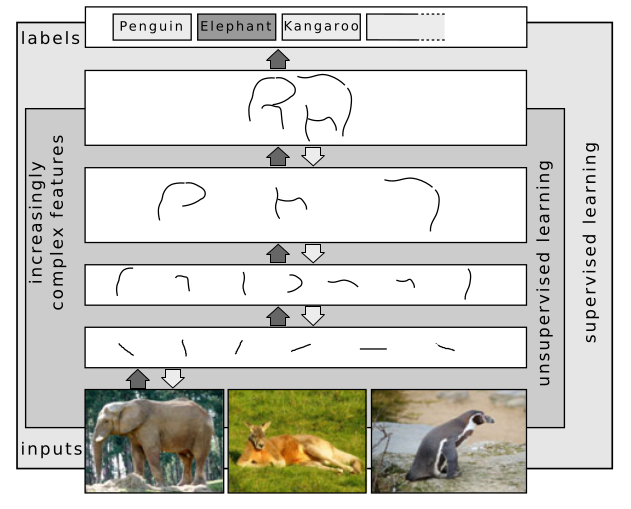
\includegraphics[width=0.7\linewidth]{figs/background/png/conv-layers.png}
    \caption{An example of extracted features from a convolutional neural network. As shown, the deeper into the network one explores, the combination of core features start to create higher level features that might represent the shape of a specific animal \cite{schulzDeepLearningLayerWise2012}.}
    \label{fig:conv-layers}
\end{figure}

Typically, these networks will downsample the image to capture the most salient information, then upsample to regenerate the features from the underlying latent representations. This network architecture has been popularized by the U-Net, which is known as a standard autoencoder (Fig. \ref{fig:unet}). Each of the layers is composed of a collection of convolution kernels, and the downsampling occurs based on the stride or size of the kernel.

\begin{figure}[h!]
    \centering
    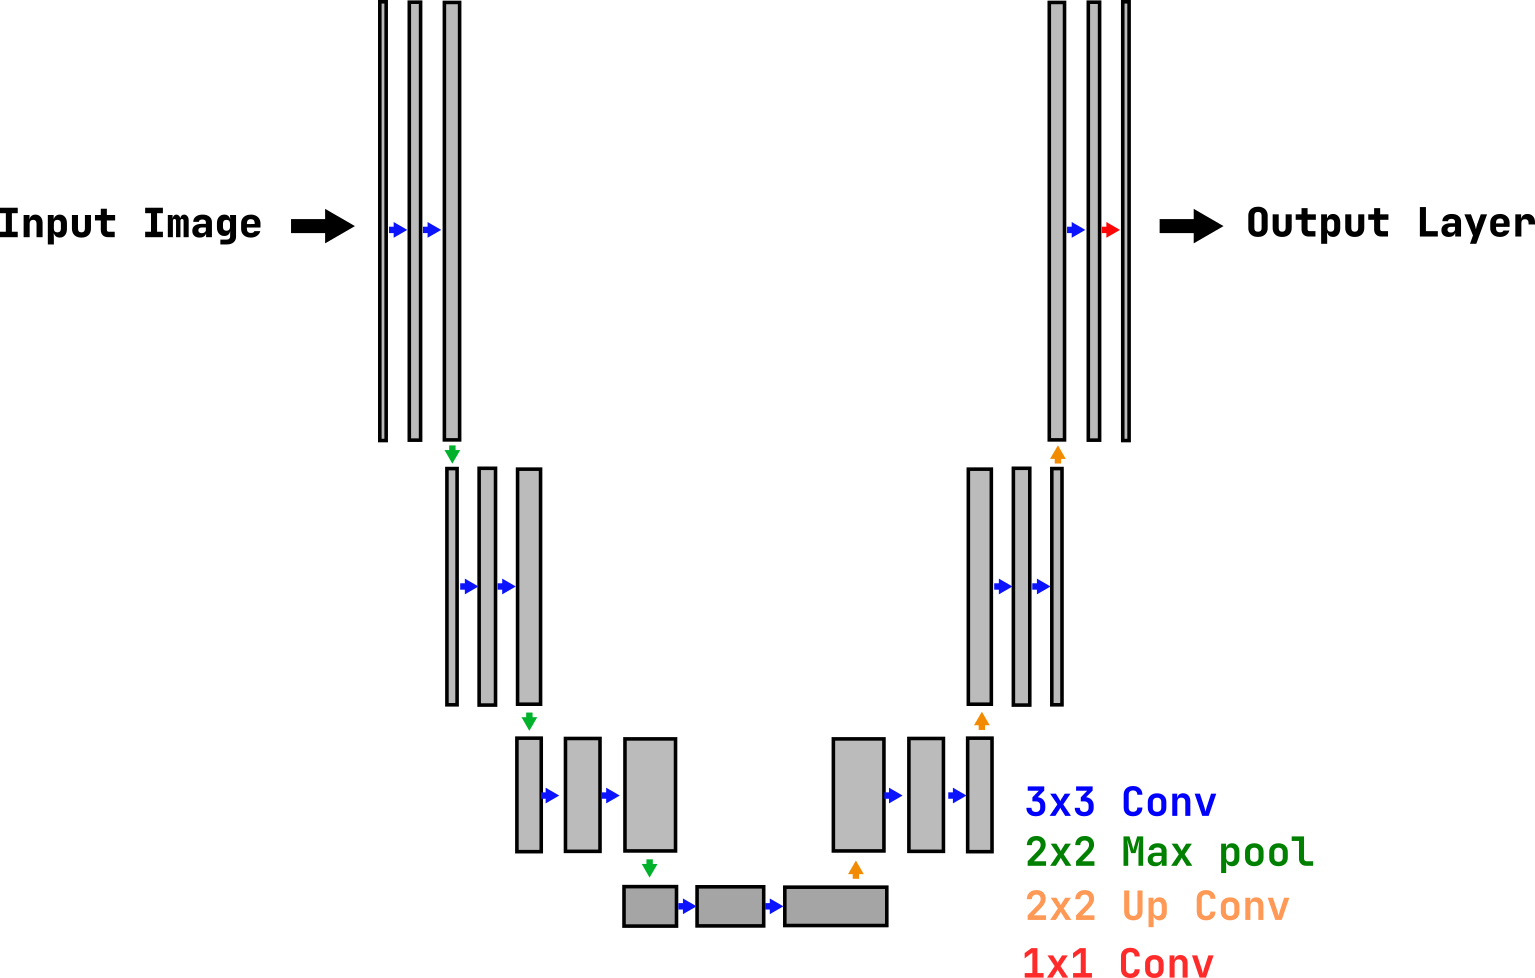
\includegraphics[width=0.7\linewidth]{figs/background/png/u-net.png}
    \caption{A standard U-Net architecture for a convolutional neural network. This architecture is the most common form of network used for biomedical image analysis and processing.}
    \label{fig:unet}
  \end{figure}


CNN architecture can be altered by changing the behavior and structure of the underlying kernels, namely size, stride, and shape. Stride controls the discrete steps the kernel takes as it is moving across the input image and can be used to downsample more aggressively. An atrous convolution involves internally padding the convolution entries with zeros. This also has the effect of more aggressively downsizing an image and capturing a larger region around the center pixel.

A convolutional neural network can have an additional fully connected network appended to the output in order to learn a mapping that involves a linear combination of the extracted features from the convolution operations. This is often used when a CNN is applied to a classification task, where the total number of outputs of the final FCN is the number of classes.

%%% Local Variables:
%%% mode: latex
%%% TeX-master: "../../../Andrew_Jensen_Dissertation"
%%% End:
